
\documentclass[11pt,a4paper]{article}
\usepackage[margin=1.9cm]{geometry}
\usepackage{amsmath,amssymb}
\usepackage{graphicx}
\usepackage{booktabs}
\usepackage{array}
\usepackage{longtable}
\usepackage{caption}
\usepackage{float}
\usepackage{hyperref}
\usepackage{xcolor}
\usepackage{enumitem}
\hypersetup{colorlinks=true, linkcolor=blue!50!black, urlcolor=blue!50!black, citecolor=blue!50!black}
\setlength{\parindent}{0pt}
\setlength{\parskip}{6pt}
\captionsetup{font=small, labelfont=bf}

\begin{document}

\begin{titlepage}
\centering
\vspace*{1.8cm}
{\Large \textbf{CE480 - HW5}\\[0.3cm]}
{\LARGE \textbf{Preliminary Small Commercial Harbor Layout and Breakwater Design}\\[0.8cm]}
\rule{0.85\textwidth}{0.6pt}\\[0.6cm]
\begin{tabular}{ll}
\textbf{Site} & Small Commercial Harbor Site (same as HW2/HW3) \\
\textbf{Coordinates} & 41.934003$^\circ$, 28.069026$^\circ$ \\
\textbf{Harbor type} & Small commercial harbor \\
\textbf{Critical wave direction} & 67.5$^\circ$ \\
\textbf{Effective fetch} & 1074.12 km \\
\end{tabular}
\vfill
\textit{Prepared from CE480 HW2, HW3, HW4 results and the confirmed HW5 assumptions.}\\[0.5cm]
\end{titlepage}

\tableofcontents
\newpage

\section{Executive Summary}
This report presents a preliminary harbor-layout and breakwater-design calculation for a small commercial harbor at the same site used in the previous CE480 homeworks. The design uses a maximum vessel length of 80 m, maximum draft of 5.5 m, and maximum beam of 14 m. A quay wall length of 150 m is adopted based on similar small commercial harbor scales.

The calculated navigation depth is \textbf{7.1 m}. The estimated bathymetry slope from the Google Earth Pro profile is \textbf{0.0196} m/m, approximately \textbf{1:51}. The required depth is reached at approximately \textbf{524 m} from the shore. Therefore, the selected perpendicular breakwater extension is \textbf{575 m}, giving a local water depth of \textbf{8.1 m} at the breakwater head/toe. The parallel arm is estimated as \textbf{400 m}, so the total preliminary breakwater length is \textbf{975 m}.

From HW4, the 10-year and 50-year deep-water design wave heights are \textbf{5.59 m} and \textbf{8.04 m}, respectively. Using the course-style Goda nearshore design-wave check at the selected breakwater depth, the corresponding design wave heights in front of the breakwater are \textbf{5.13 m} and \textbf{5.38 m}. The governing condition is depth-limited breaking.

\section{Problem Statement and Methodology}
The homework requires the harbor dimensions and wave-design checks listed below:
\begin{enumerate}[leftmargin=1.0cm]
    \item Select representative maximum and mean ship sizes for the selected harbor type.
    \item Estimate quay wall or pier length from similar harbor scale.
    \item Calculate the turning basin.
    \item Determine the breakwater extension perpendicular and parallel to shore.
    \item Determine the necessary water depth using a navigation-channel depth formula.
    \item Check whether the breakwater reaches the required depth; if not, propose a navigation channel.
    \item Use HW4 10-year and 50-year deep-water wave heights and calculate the design wave height in front of the breakwater using Goda's formula with wave steepness $s_0=0.04$.
\end{enumerate}

The workflow is summarized as follows:
\[
\text{Ship size} \rightarrow \text{quay and basin dimensions} \rightarrow \text{navigation depth} \rightarrow \text{breakwater reach} \rightarrow \text{Goda design wave}
\]

\section{Input Data and Assumptions}
\subsection{Site and wave inputs}
The site and wave inputs are taken from the previous CE480 homework workflow. The critical wave direction is the direction with the largest effective fetch. The fetch and wave-return values are treated as fixed inputs for this HW5 preliminary design.

\begin{table}[H]
\centering
\caption{Main input data used in HW5.}
\begin{tabular}{lll}
\toprule
\textbf{Input} & \textbf{Value} & \textbf{Unit} \\
\midrule
Site latitude & 41.934003 & deg \\
Site longitude & 28.069026 & deg \\
Harbor type & Small commercial harbor & - \\
Critical wave direction & 67.5 & deg \\
Effective fetch & 1074.12 & km \\
Deep-water wave steepness, $s_0$ & 0.04 & - \\
Bathymetry point 1 & 457.2 m, depth 5.79 m & - \\
Bathymetry point 2 & 2027.8 m, depth 36.58 m & - \\
Estimated seabed slope & 0.0196 & m/m \\
Approximate seabed slope & 1:51 & - \\
\bottomrule
\end{tabular}
\end{table}

\subsection{Design vessel and quay assumptions}
For a small commercial harbor, the design vessel was selected as a small general-cargo/coaster-type vessel. Since no specific vessel fleet was assigned in the homework statement, the values below are preliminary assumptions and should be replaced if the instructor requires a specific vessel type.

\begin{table}[H]
\centering
\caption{Design vessel, quay, and harbor-basin assumptions.}
\begin{tabular}{lll}
\toprule
\textbf{Item} & \textbf{Value} & \textbf{Unit} \\
\midrule
Mean ship length & 50 & m \\
Maximum/design ship length, $L_{max}$ & 80 & m \\
Mean draft & 4.0 & m \\
Maximum/design draft, $T_d$ & 5.5 & m \\
Mean beam & 9 & m \\
Maximum/design beam, $B_{max}$ & 14 & m \\
Quay wall length & 150 & m \\
Entrance width & 100 & m \\
\bottomrule
\end{tabular}
\end{table}

\section{Turning Basin, Channel Width, and Quay Length}
The turning basin diameter is taken as twice the maximum design vessel length:
\begin{equation}
D_T = 2L_{max}
\end{equation}
\begin{equation}
D_T = 2(80) = 160\ \mathrm{m}
\end{equation}

The one-way preliminary navigation channel width is estimated as:
\begin{equation}
B_c = 5B_{max}
\end{equation}
\begin{equation}
B_c = 5(14) = 70\ \mathrm{m}
\end{equation}

The adopted quay wall length is 150 m. This provides berthing space for approximately one small commercial vessel with operational allowance, or a shorter combination of small service vessels.

\section{Navigation Depth Calculation}
The required navigation depth is computed by adding the design draft, under-keel clearance, wave allowance, dredging tolerance, and sedimentation allowance:
\begin{equation}
D_{req} = T_d + UKC + A_w + A_d + A_s
\end{equation}
where $T_d$ is the design vessel draft, $UKC$ is under-keel clearance, $A_w$ is wave allowance, $A_d$ is dredging tolerance, and $A_s$ is sedimentation allowance.

The under-keel clearance is assumed as 10\% of the design draft:
\begin{equation}
UKC = 0.10T_d = 0.10(5.5) = 0.55\ \mathrm{m}
\end{equation}
Therefore,
\begin{equation}
D_{req} = 5.5 + 0.55 + 0.50 + 0.30 + 0.20 = 7.05\ \mathrm{m}
\end{equation}
After rounding upward, the adopted required navigation depth is:
\begin{equation}
\boxed{D_{req} = 7.1\ \mathrm{m}}
\end{equation}

\begin{table}[H]
\centering
\caption{Navigation depth calculation.}
\begin{tabular}{lr}
\toprule
\textbf{Component} & \textbf{Value (m)} \\
\midrule
Design draft & 5.50 \\
Under-keel clearance (10\% draft) & 0.55 \\
Wave allowance & 0.50 \\
Dredging tolerance & 0.30 \\
Sedimentation allowance & 0.20 \\
Required depth before rounding & 7.05 \\
\textbf{Required design depth} & \textbf{7.10} \\
\bottomrule
\end{tabular}
\end{table}

\begin{figure}[H]
\centering
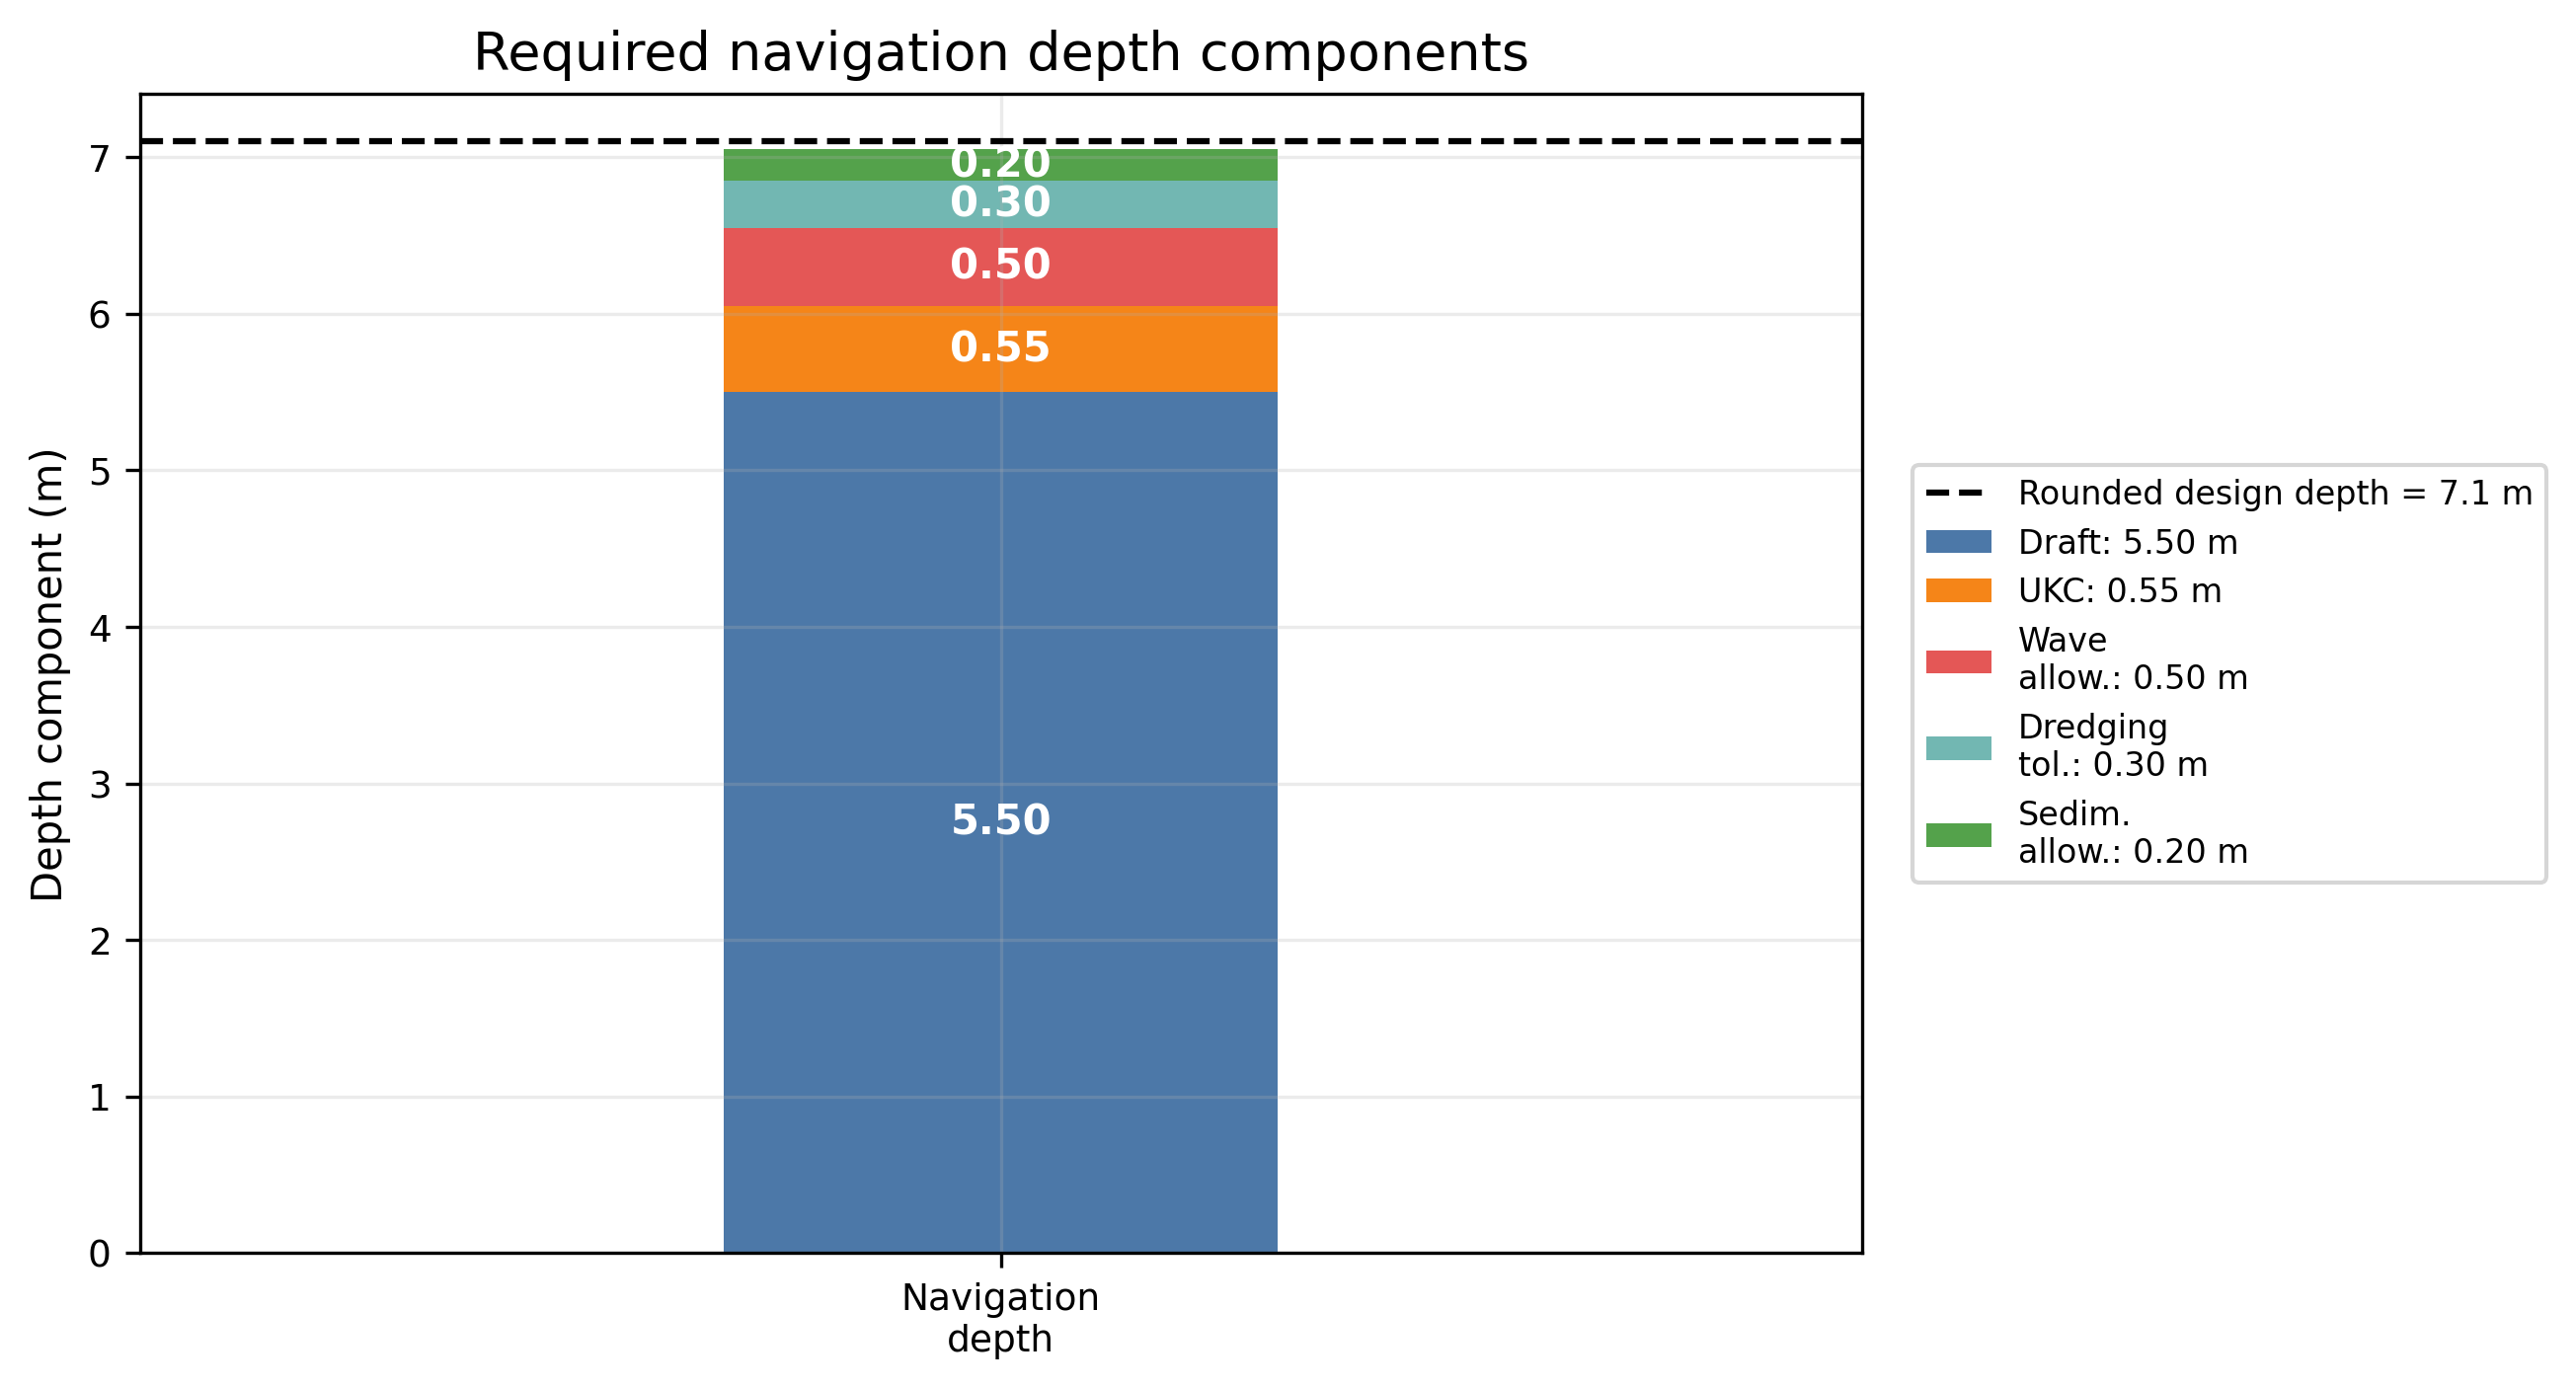
\includegraphics[width=0.92\textwidth]{figures/fig_3_navigation_depth_components.png}
\caption{Components of the required navigation depth.}
\end{figure}

\section{Bathymetry, Required Depth, and Breakwater Reach}
The Google Earth Pro profile points were converted from English units to SI units. A linear bathymetry model was fitted between the two points:
\begin{equation}
h(x)=h_0+mx
\end{equation}
where $x$ is offshore distance and $h$ is water depth. The estimated slope is:
\begin{equation}
m = \frac{36.58-5.79}{2027.8-457.2} = 0.0196\ \approx 1:51
\end{equation}

The distance where the required depth is reached is:
\begin{equation}
x_{req} = \frac{D_{req}-h_0}{m} = 524\ \mathrm{m}
\end{equation}

To ensure the breakwater reaches slightly deeper water than the minimum navigation requirement, an additional 50 m is added and the result is rounded up:
\begin{equation}
L_{BW,\perp} = \mathrm{round\ up}(x_{req}+50) = 575\ \mathrm{m}
\end{equation}
The resulting depth at the breakwater head/toe is approximately:
\begin{equation}
h_{toe} = 8.1\ \mathrm{m}
\end{equation}

\begin{figure}[H]
\centering
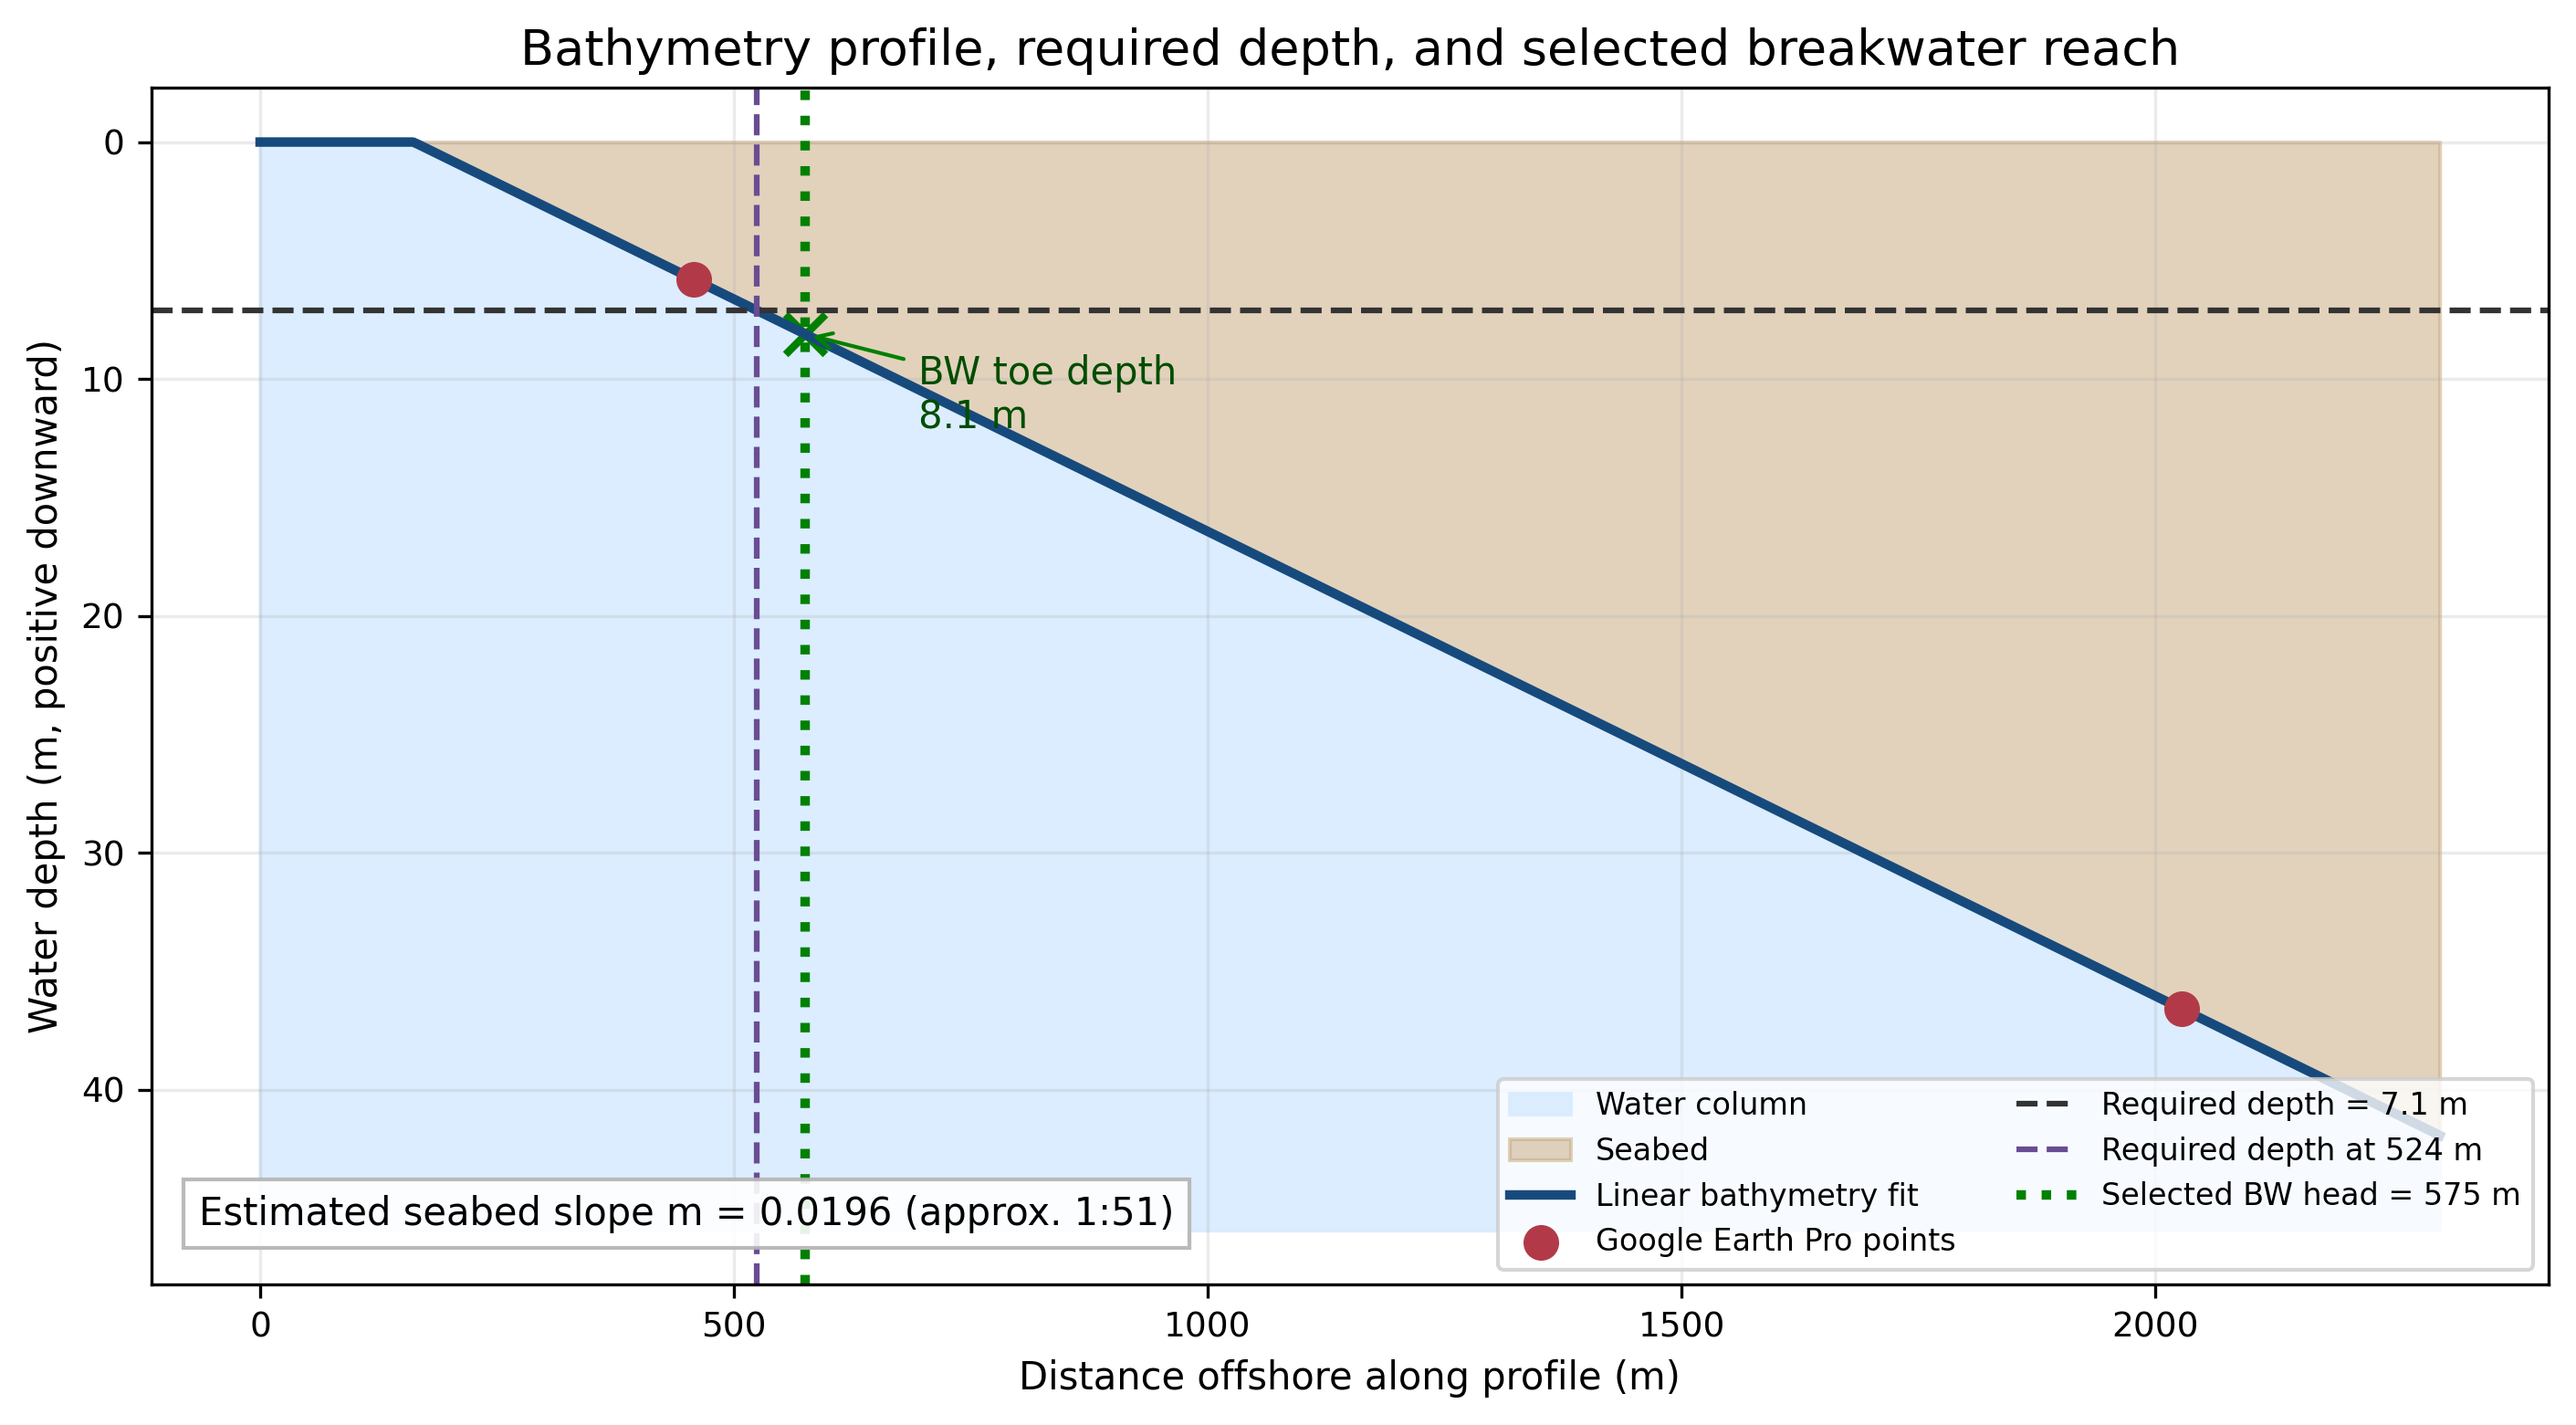
\includegraphics[width=0.96\textwidth]{figures/fig_1_bathymetry_profile_enhanced.png}
\caption{Bathymetry profile, required navigation depth, and selected breakwater head distance.}
\end{figure}

\section{Breakwater Layout}
The preliminary breakwater layout is composed of two parts:
\begin{enumerate}[leftmargin=1.0cm]
    \item A perpendicular arm extending from shore until the required water depth is exceeded.
    \item A parallel arm protecting the quay and turning basin from the critical wave direction.
\end{enumerate}

The parallel breakwater length is estimated from the quay length, turning basin diameter, and an additional protection margin:
\begin{equation}
L_{BW,\parallel} = L_q + D_T + M_p
\end{equation}
\begin{equation}
L_{BW,\parallel} = 150 + 160 + 80 = 390\ \mathrm{m} \approx 400\ \mathrm{m}
\end{equation}
Thus, the total preliminary breakwater length is:
\begin{equation}
L_{BW,total} = 575+400=975\ \mathrm{m}
\end{equation}

\begin{table}[H]
\centering
\caption{Summary of harbor layout dimensions.}
\begin{tabular}{lrl}
\toprule
\textbf{Item} & \textbf{Value} & \textbf{Unit} \\
\midrule
Turning basin diameter & 160 & m \\
Channel width & 70 & m \\
Required navigation depth & 7.1 & m \\
Distance to required depth & 524 & m from shoreline \\
Perpendicular breakwater length & 575 & m \\
Depth at breakwater head/toe & 8.1 & m \\
Parallel breakwater length & 400 & m \\
\textbf{Total breakwater length} & \textbf{975} & \textbf{m} \\
\bottomrule
\end{tabular}
\end{table}

\begin{figure}[H]
\centering
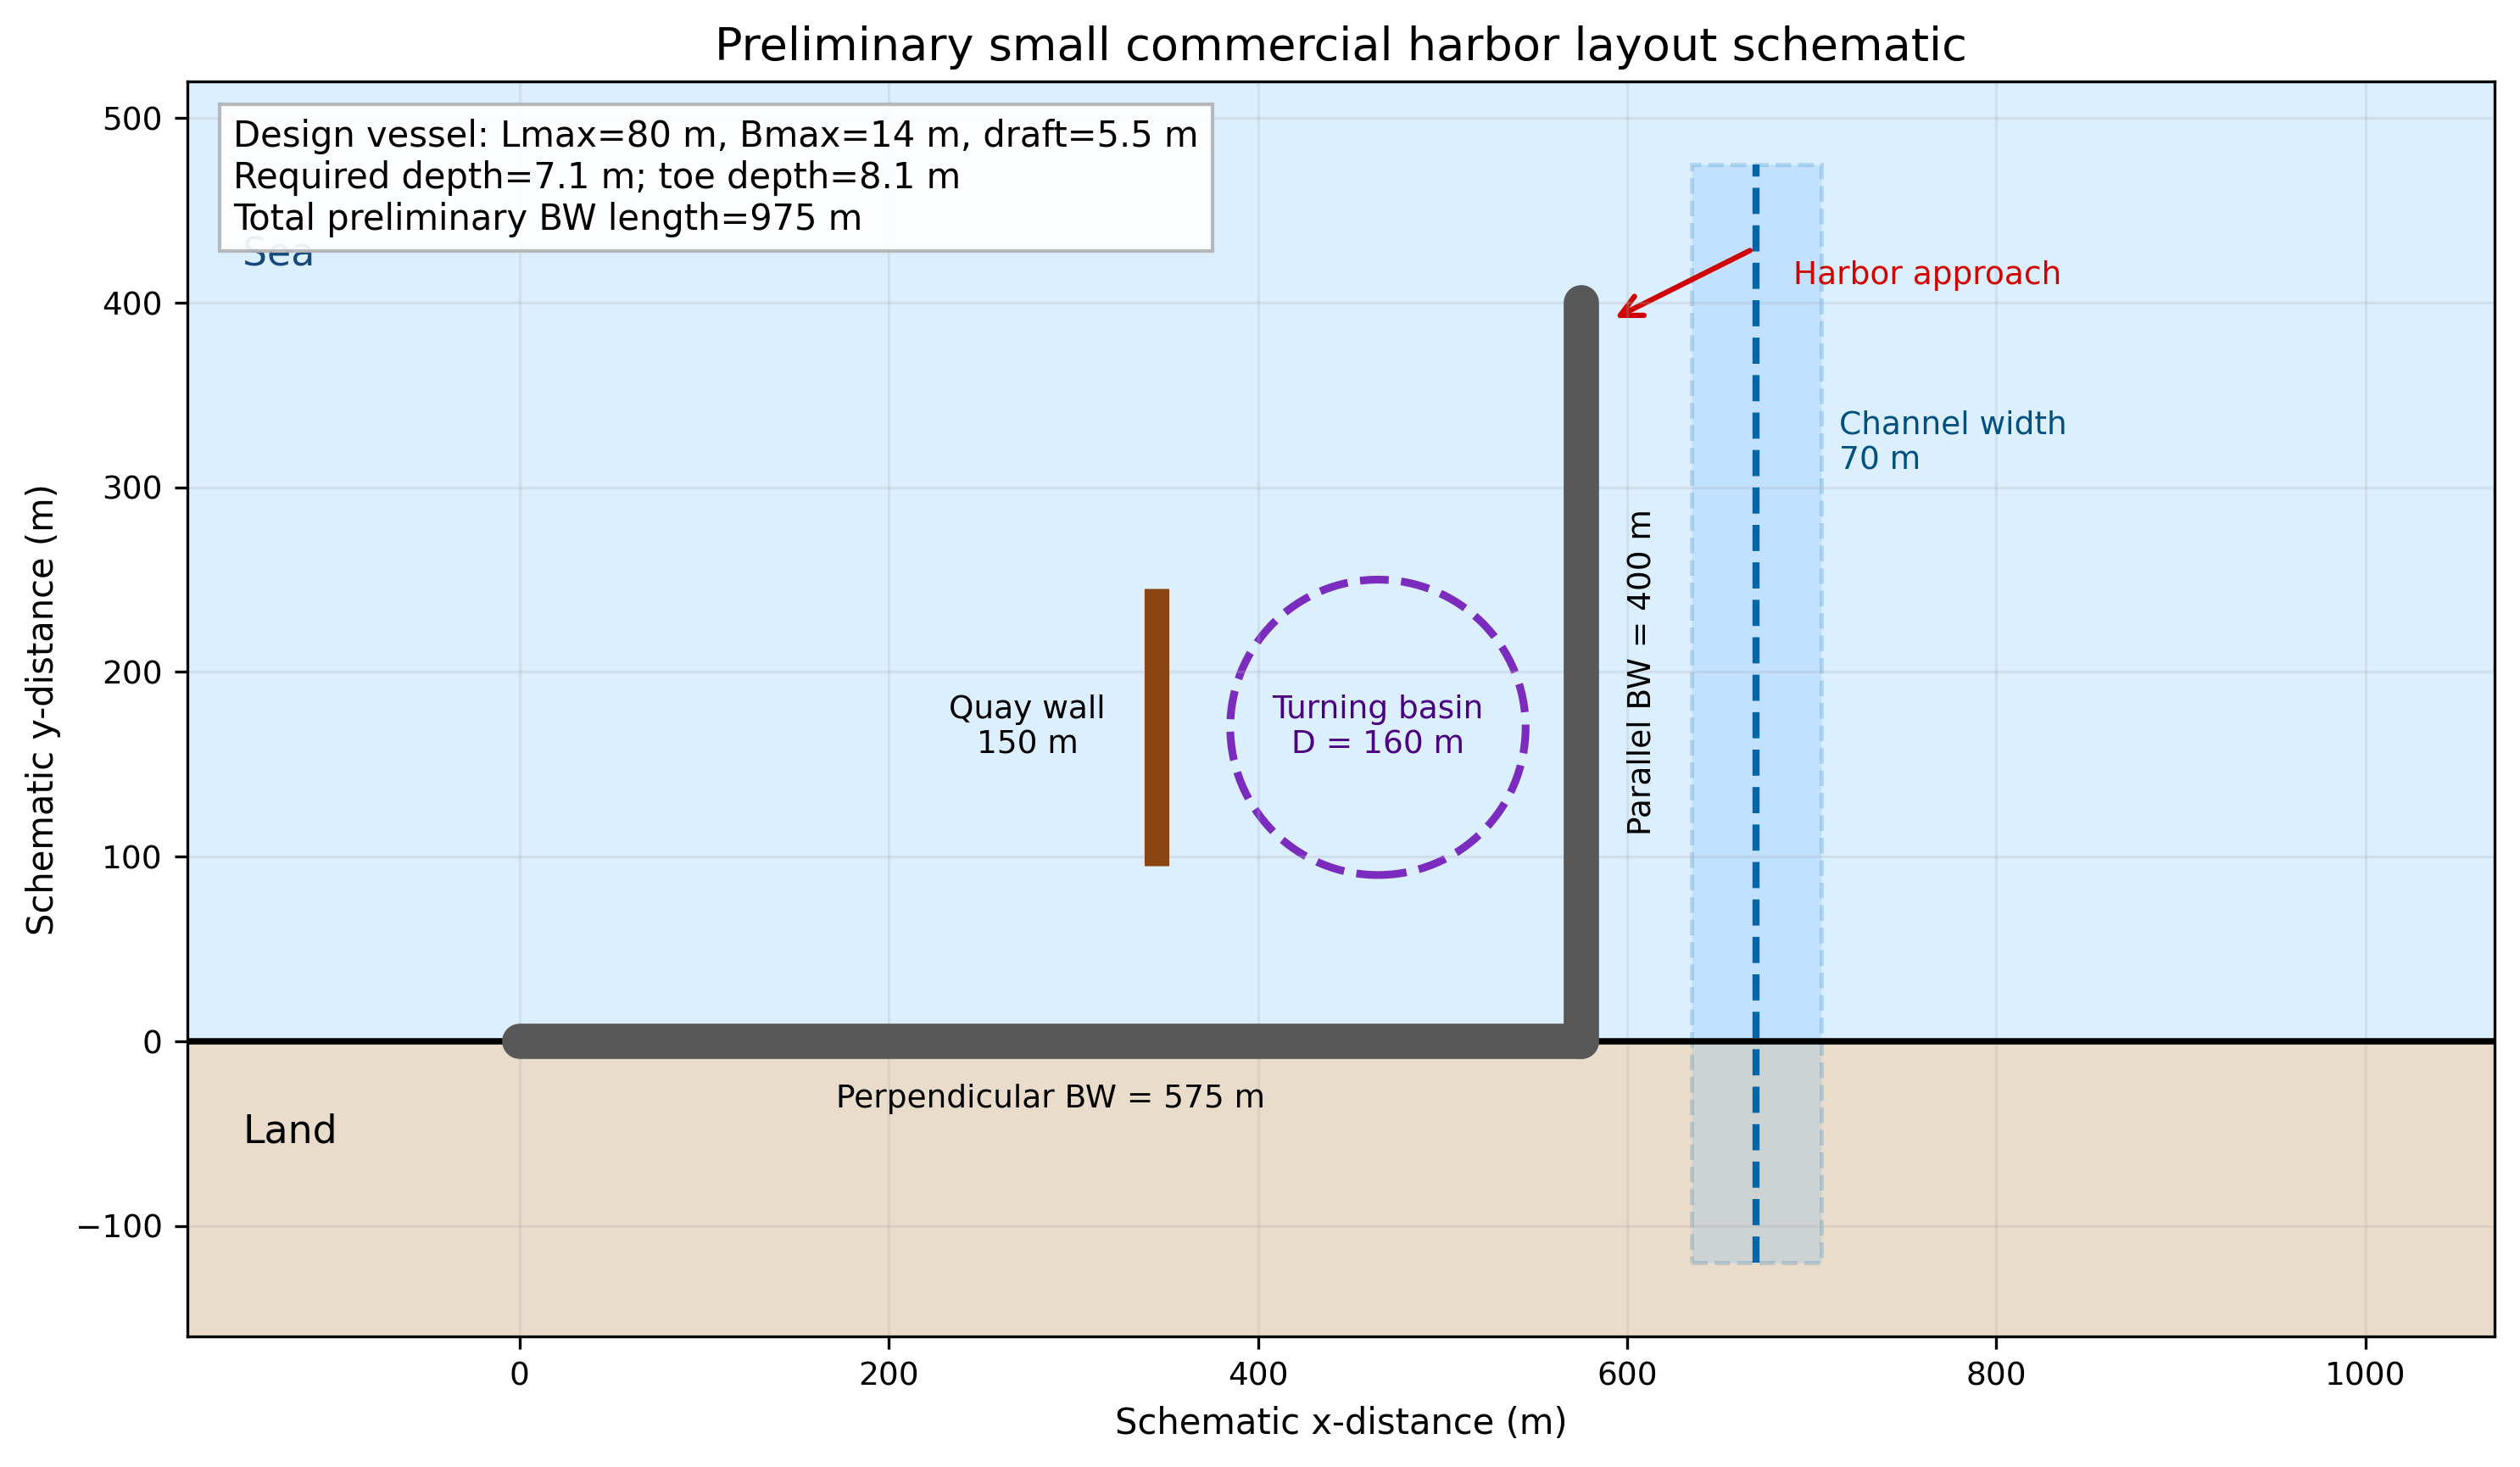
\includegraphics[width=0.96\textwidth]{figures/fig_2_harbor_layout_enhanced.png}
\caption{Preliminary harbor layout schematic. The figure is a conceptual layout, not a georeferenced engineering drawing.}
\end{figure}

\section{Deep-Water Design Waves from HW4}
The deep-water return wave heights were obtained using the Gumbel extreme-value method. The plotting position used in the previous HW4 code is the Gringorten form:
\begin{equation}
P = 1 - \frac{m-C_1}{N+C_2}, \quad C_1=0.44, \quad C_2=0.12
\end{equation}
where $m$ is rank and $N$ is the number of annual maxima. The Gumbel reduced variate is:
\begin{equation}
y=-\ln[-\ln(P)]
\end{equation}
The fitted relation is:
\begin{equation}
H_s = ay+b = 1.4849y + 2.2476, \quad R^2=0.969
\end{equation}

For a return period $T_R$, the exceedance probability is $Q=1/T_R$ and the non-exceedance probability is $P=1-Q$.

\begin{table}[H]
\centering
\caption{Deep-water return-period wave heights used in HW5.}
\begin{tabular}{rrrr}
\toprule
\textbf{$T_R$ (yr)} & \textbf{$P$} & \textbf{$y$} & \textbf{$H_0$ (m)} \\
\midrule
10 & 0.900 & 2.250 & 5.59 \\
50 & 0.980 & 3.902 & 8.04 \\
100 & 0.990 & 4.600 & 9.08 \\
\bottomrule
\end{tabular}
\end{table}

\begin{figure}[H]
\centering
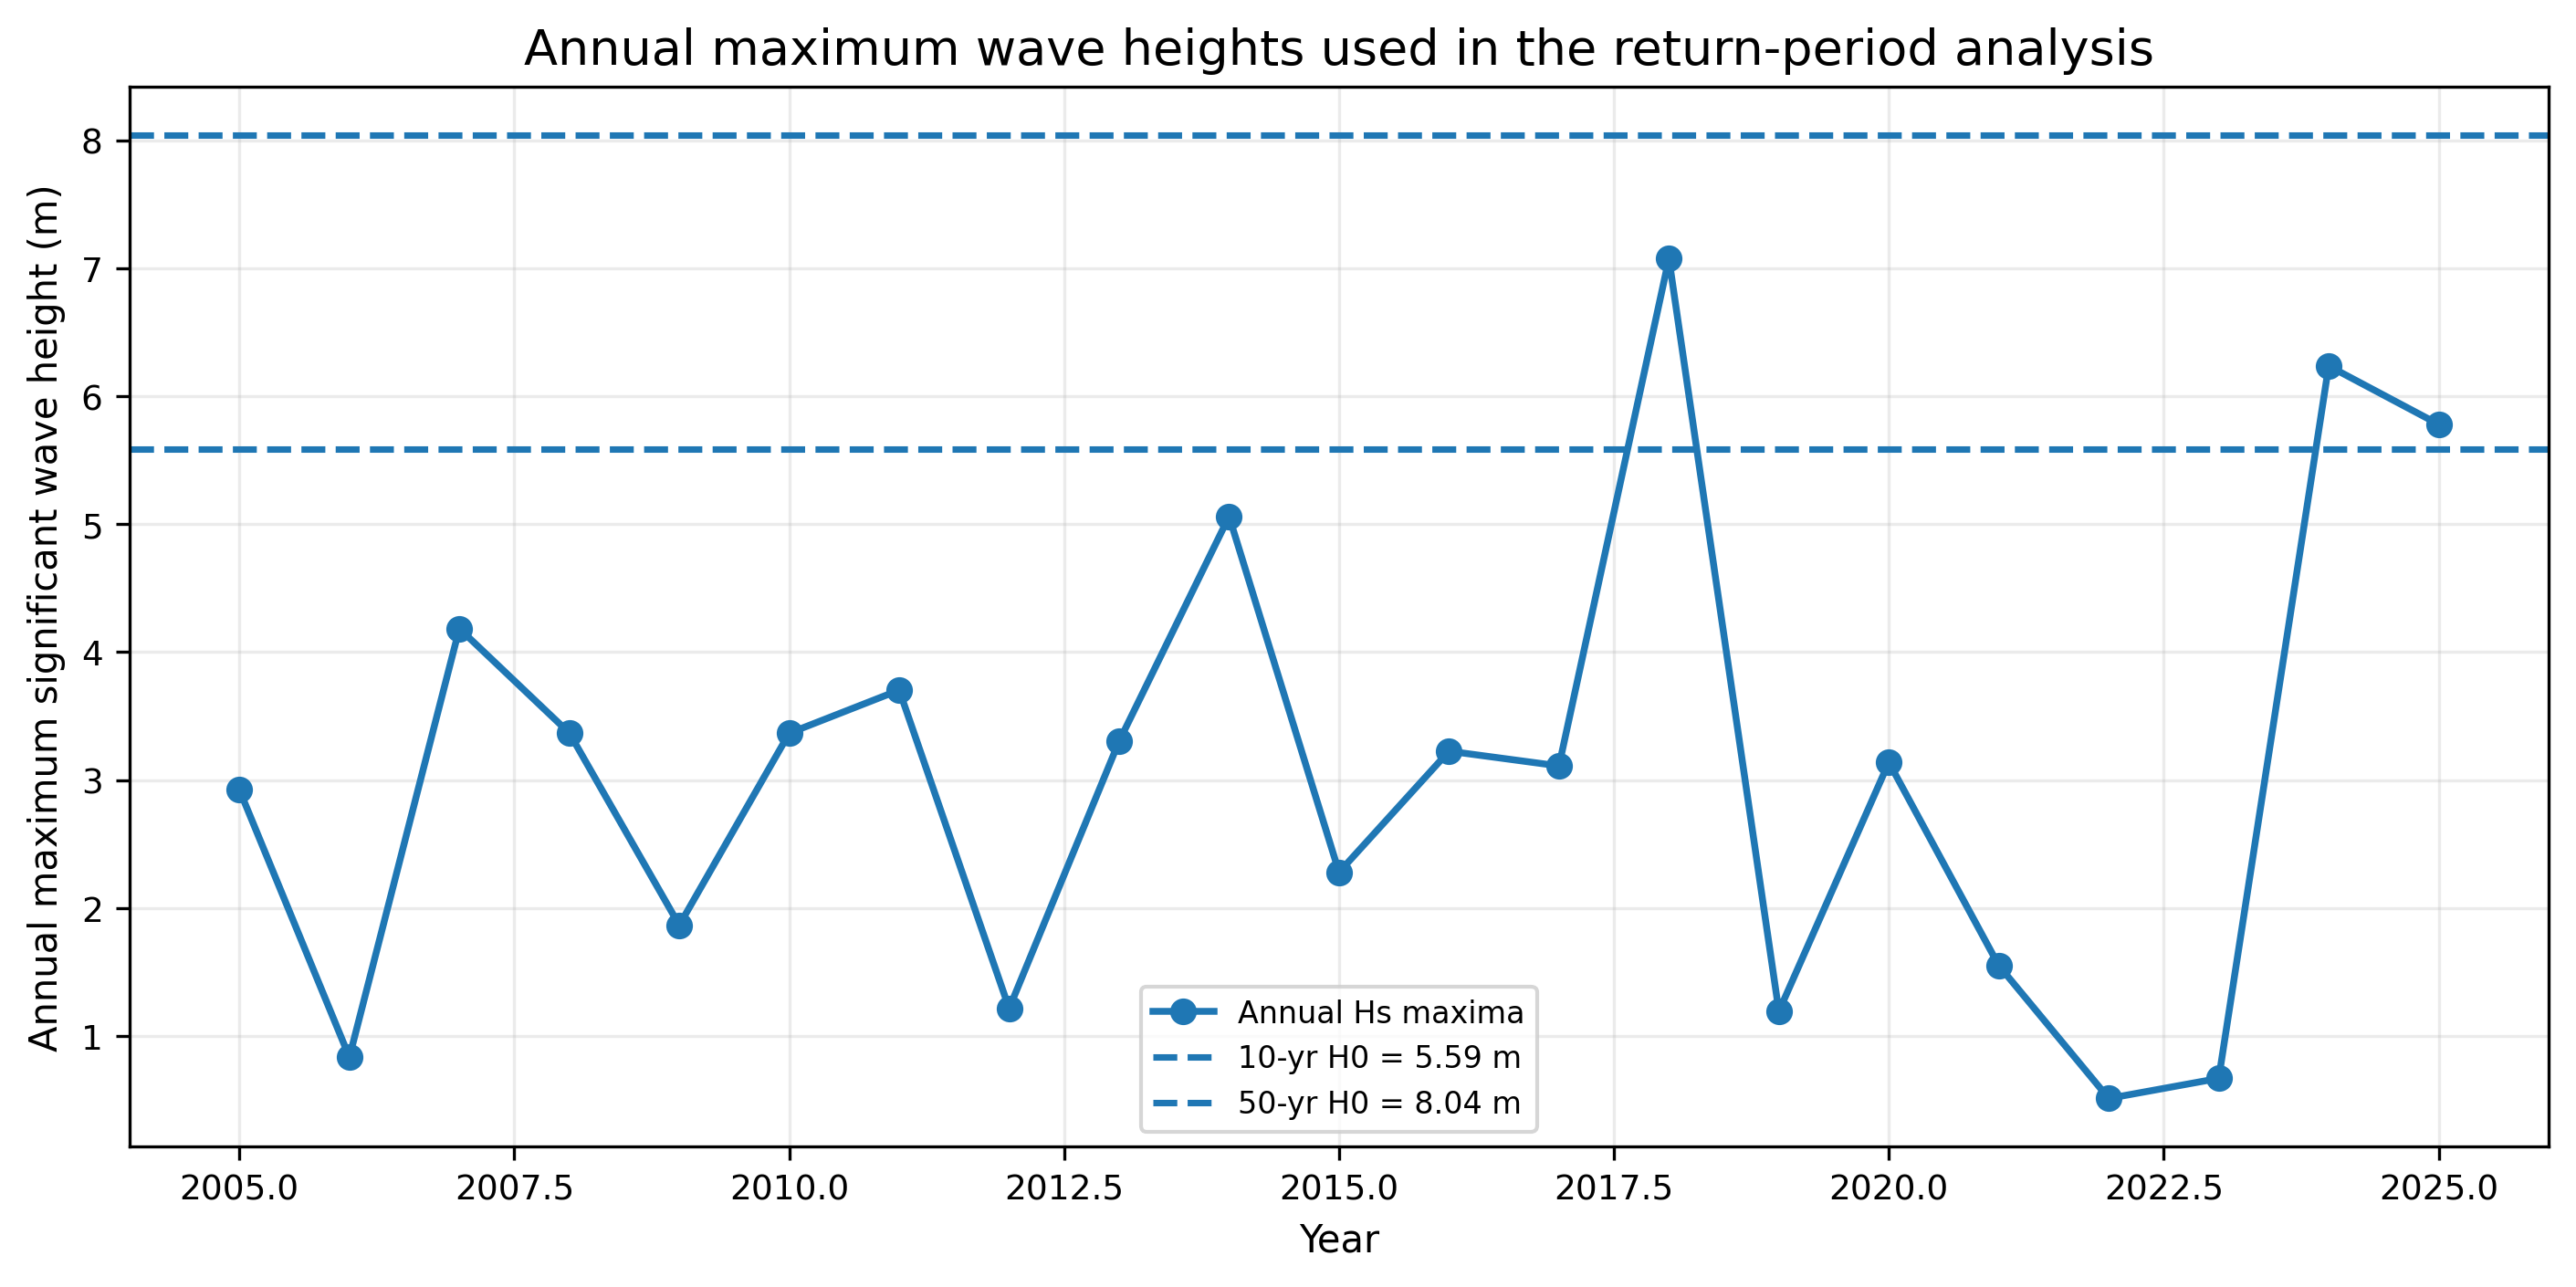
\includegraphics[width=0.94\textwidth]{figures/fig_5_annual_hs_timeseries.png}
\caption{Annual maximum significant wave heights and 10-year/50-year return wave levels.}
\end{figure}

\begin{figure}[H]
\centering
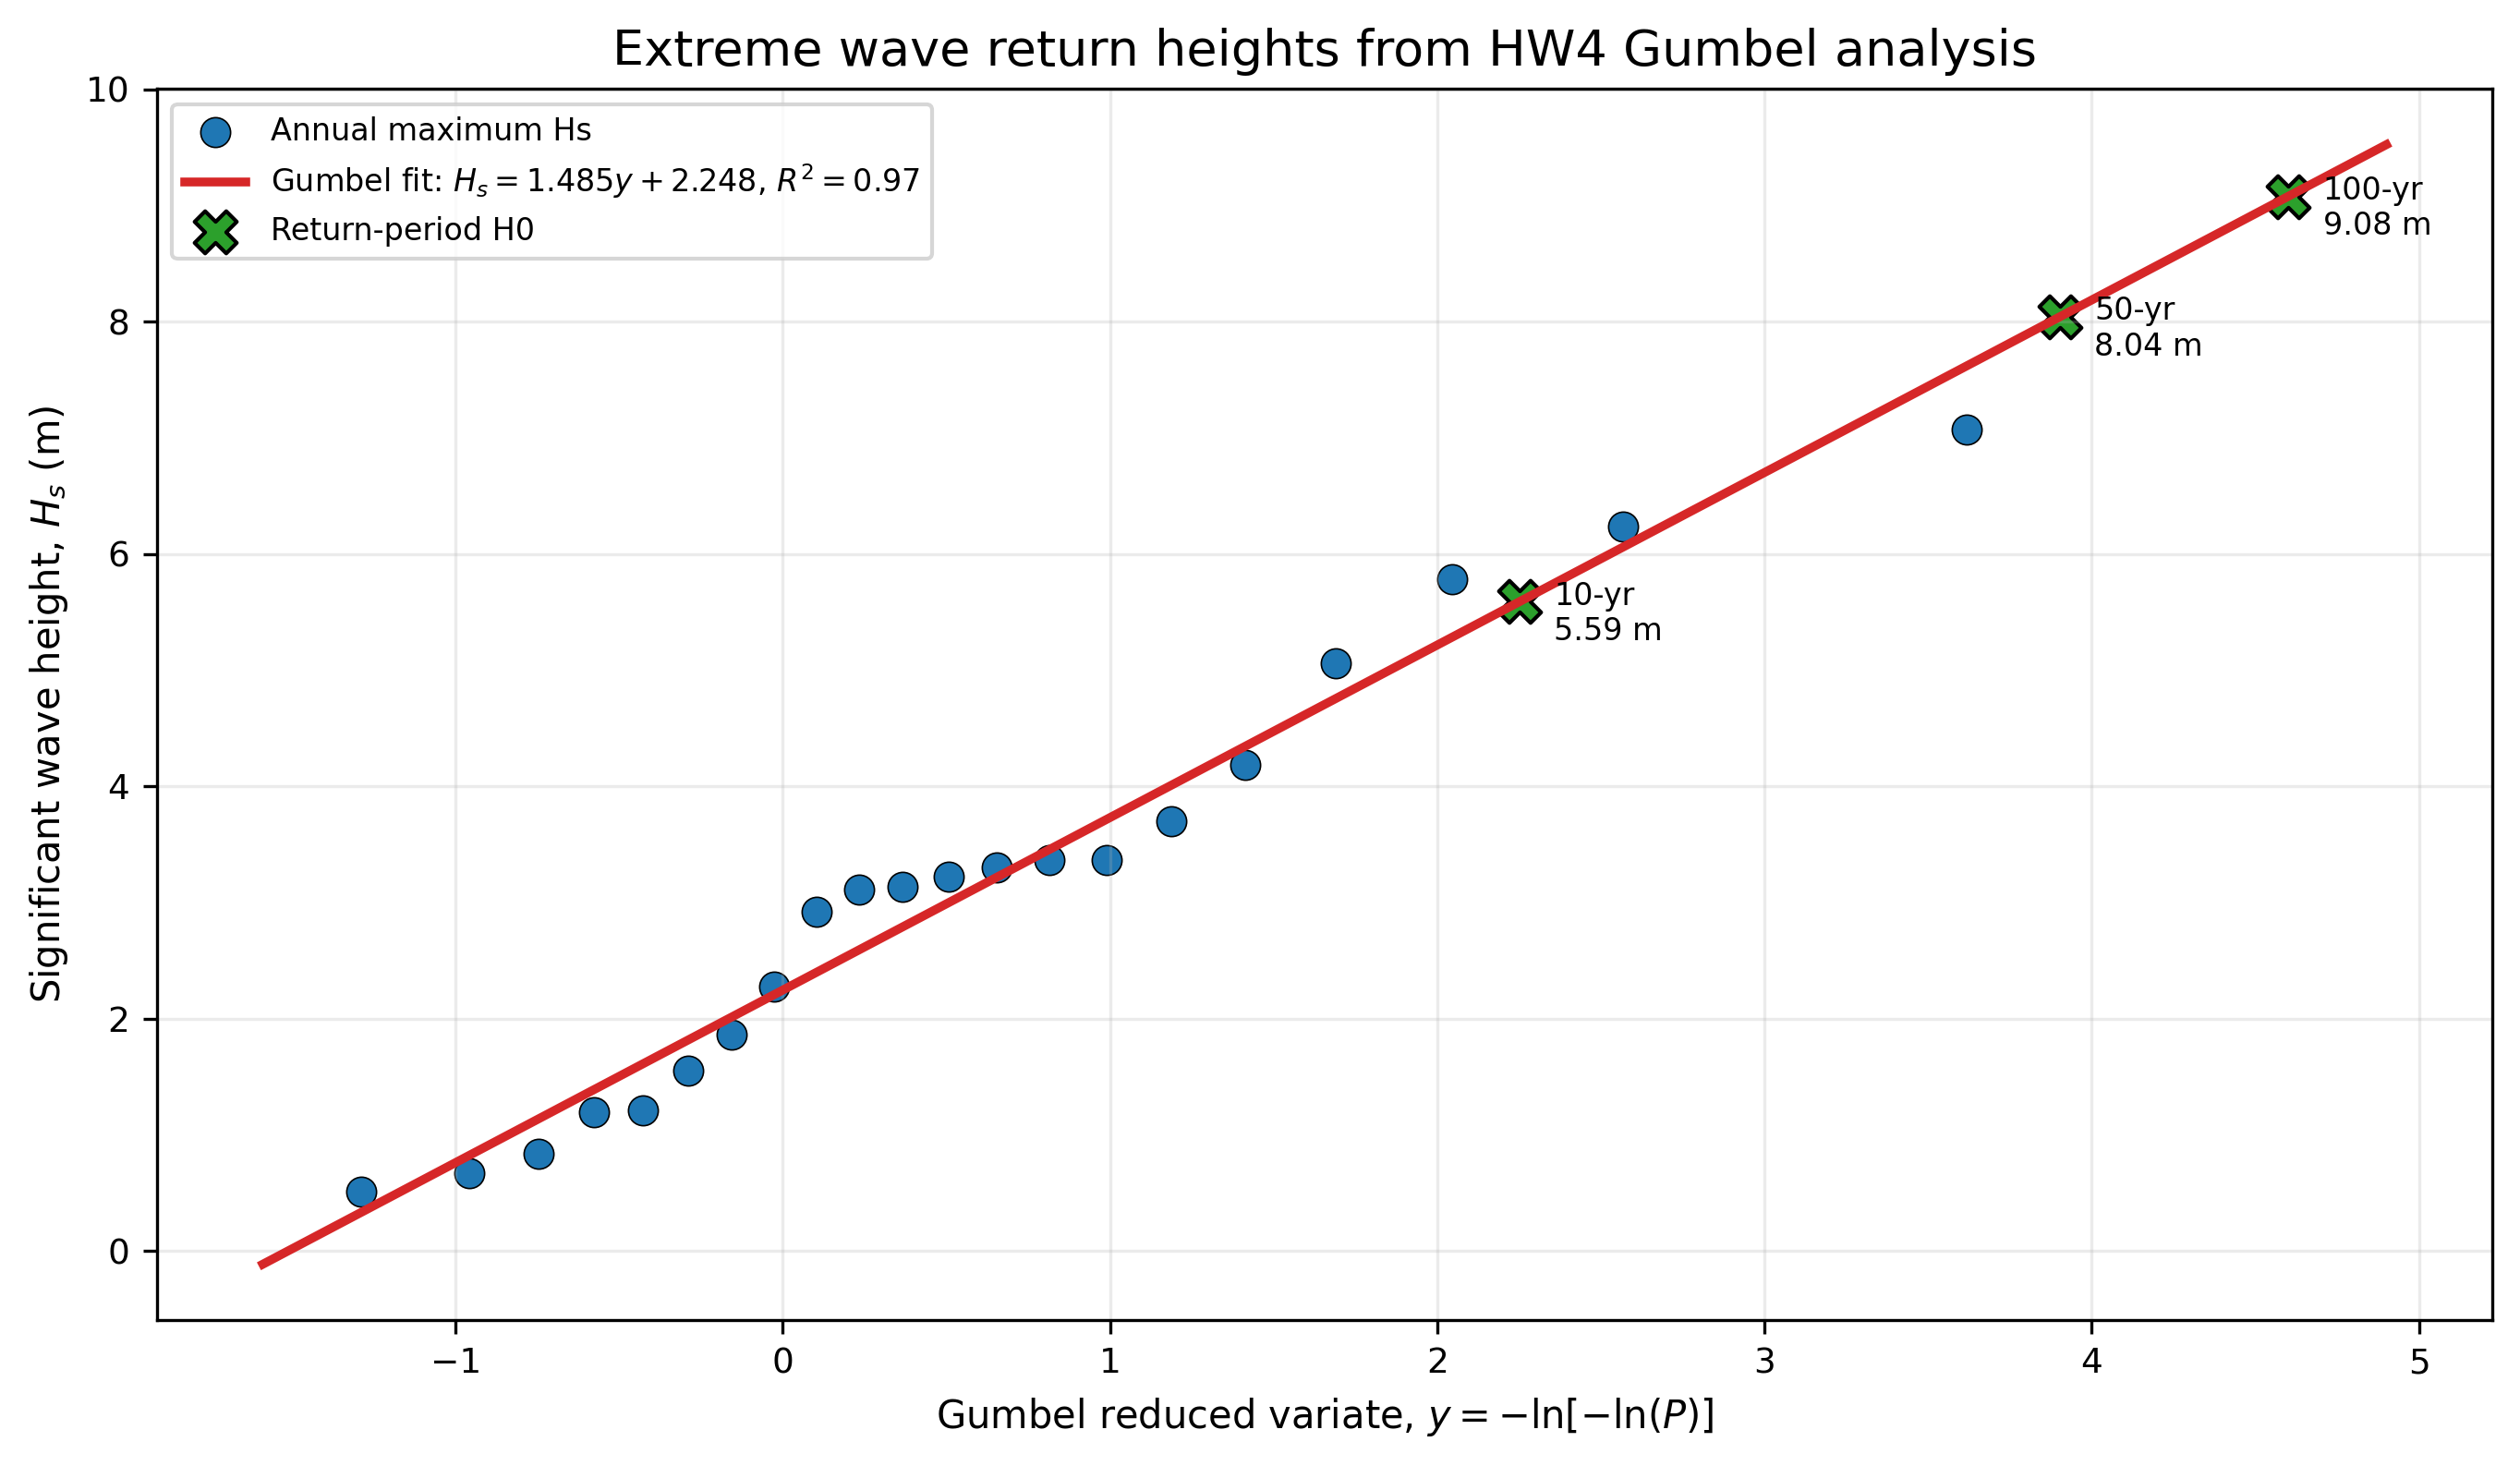
\includegraphics[width=0.94\textwidth]{figures/fig_4_gumbel_return_heights_enhanced.png}
\caption{Gumbel fit and return-period wave heights.}
\end{figure}

\section{Goda Design Wave Height at the Breakwater}
The design wave height in front of the breakwater is evaluated at the local depth $h=8.1$ m. The wave steepness is given by the homework statement as:
\begin{equation}
s_0=\frac{H_0}{L_0}=0.04
\end{equation}
Therefore, for each return-period wave:
\begin{equation}
L_0=\frac{H_0}{s_0}
\end{equation}
and the wave period is obtained from the deep-water dispersion relation:
\begin{equation}
L_0=\frac{gT^2}{2\pi} \quad \Rightarrow \quad T=\sqrt{\frac{2\pi L_0}{g}}
\end{equation}

The course-style Goda nearshore wave-height check is implemented as:
\begin{equation}
H_d = \min\left(K_sH_0,\ \beta_0H_0+\beta_1h,\ \beta_{max}H_0\right)
\end{equation}
where $K_s$ is the shoaling coefficient, $h$ is the local water depth, and the $\beta$ coefficients depend on wave steepness and seabed slope. The coefficient set used in the calculation is:
\begin{align}
\beta_0 &= 0.028s_0^{-0.38}\exp(20m^{1.5}) \\
\beta_1 &= 0.52\exp(4.2m) \\
\beta_{max} &= \max\left[0.92,\ 0.32s_0^{-0.29}\exp(2.4m)\right]
\end{align}
where $m=0.0196$ is the seabed slope. The selected design wave is the smallest of the three candidate terms because it represents the limiting transformation/breaking condition at the breakwater location.

\begin{table}[H]
\centering
\caption{Goda-type design wave calculation results.}
\begin{tabular}{rrrrrl}
\toprule
\textbf{$T_R$ (yr)} & \textbf{$H_0$ (m)} & \textbf{$T$ (s)} & \textbf{$h$ (m)} & \textbf{$H_d$ (m)} & \textbf{Governing condition} \\
\midrule
10 & 5.59 & 9.46 & 8.10 & 5.13 & Depth-limited breaking \\
50 & 8.04 & 11.35 & 8.10 & 5.38 & Depth-limited breaking \\
100 & 9.08 & 12.06 & 8.10 & 5.49 & Depth-limited breaking \\
\bottomrule
\end{tabular}
\end{table}

\begin{table}[H]
\centering
\caption{Candidate terms in Goda design wave calculation.}
\begin{tabular}{rrrrr}
\toprule
\textbf{$T_R$ (yr)} & \textbf{$K_sH_0$ (m)} & \textbf{$\beta_0H_0+\beta_1h$ (m)} & \textbf{$\beta_{max}H_0$ (m)} & \textbf{Selected $H_d$ (m)} \\
\midrule
10 & 5.58 & 5.13 & 5.14 & 5.13 \\
50 & 8.55 & 5.38 & 7.40 & 5.38 \\
100 & 9.87 & 5.49 & 8.35 & 5.49 \\
\bottomrule
\end{tabular}
\end{table}

\begin{figure}[H]
\centering
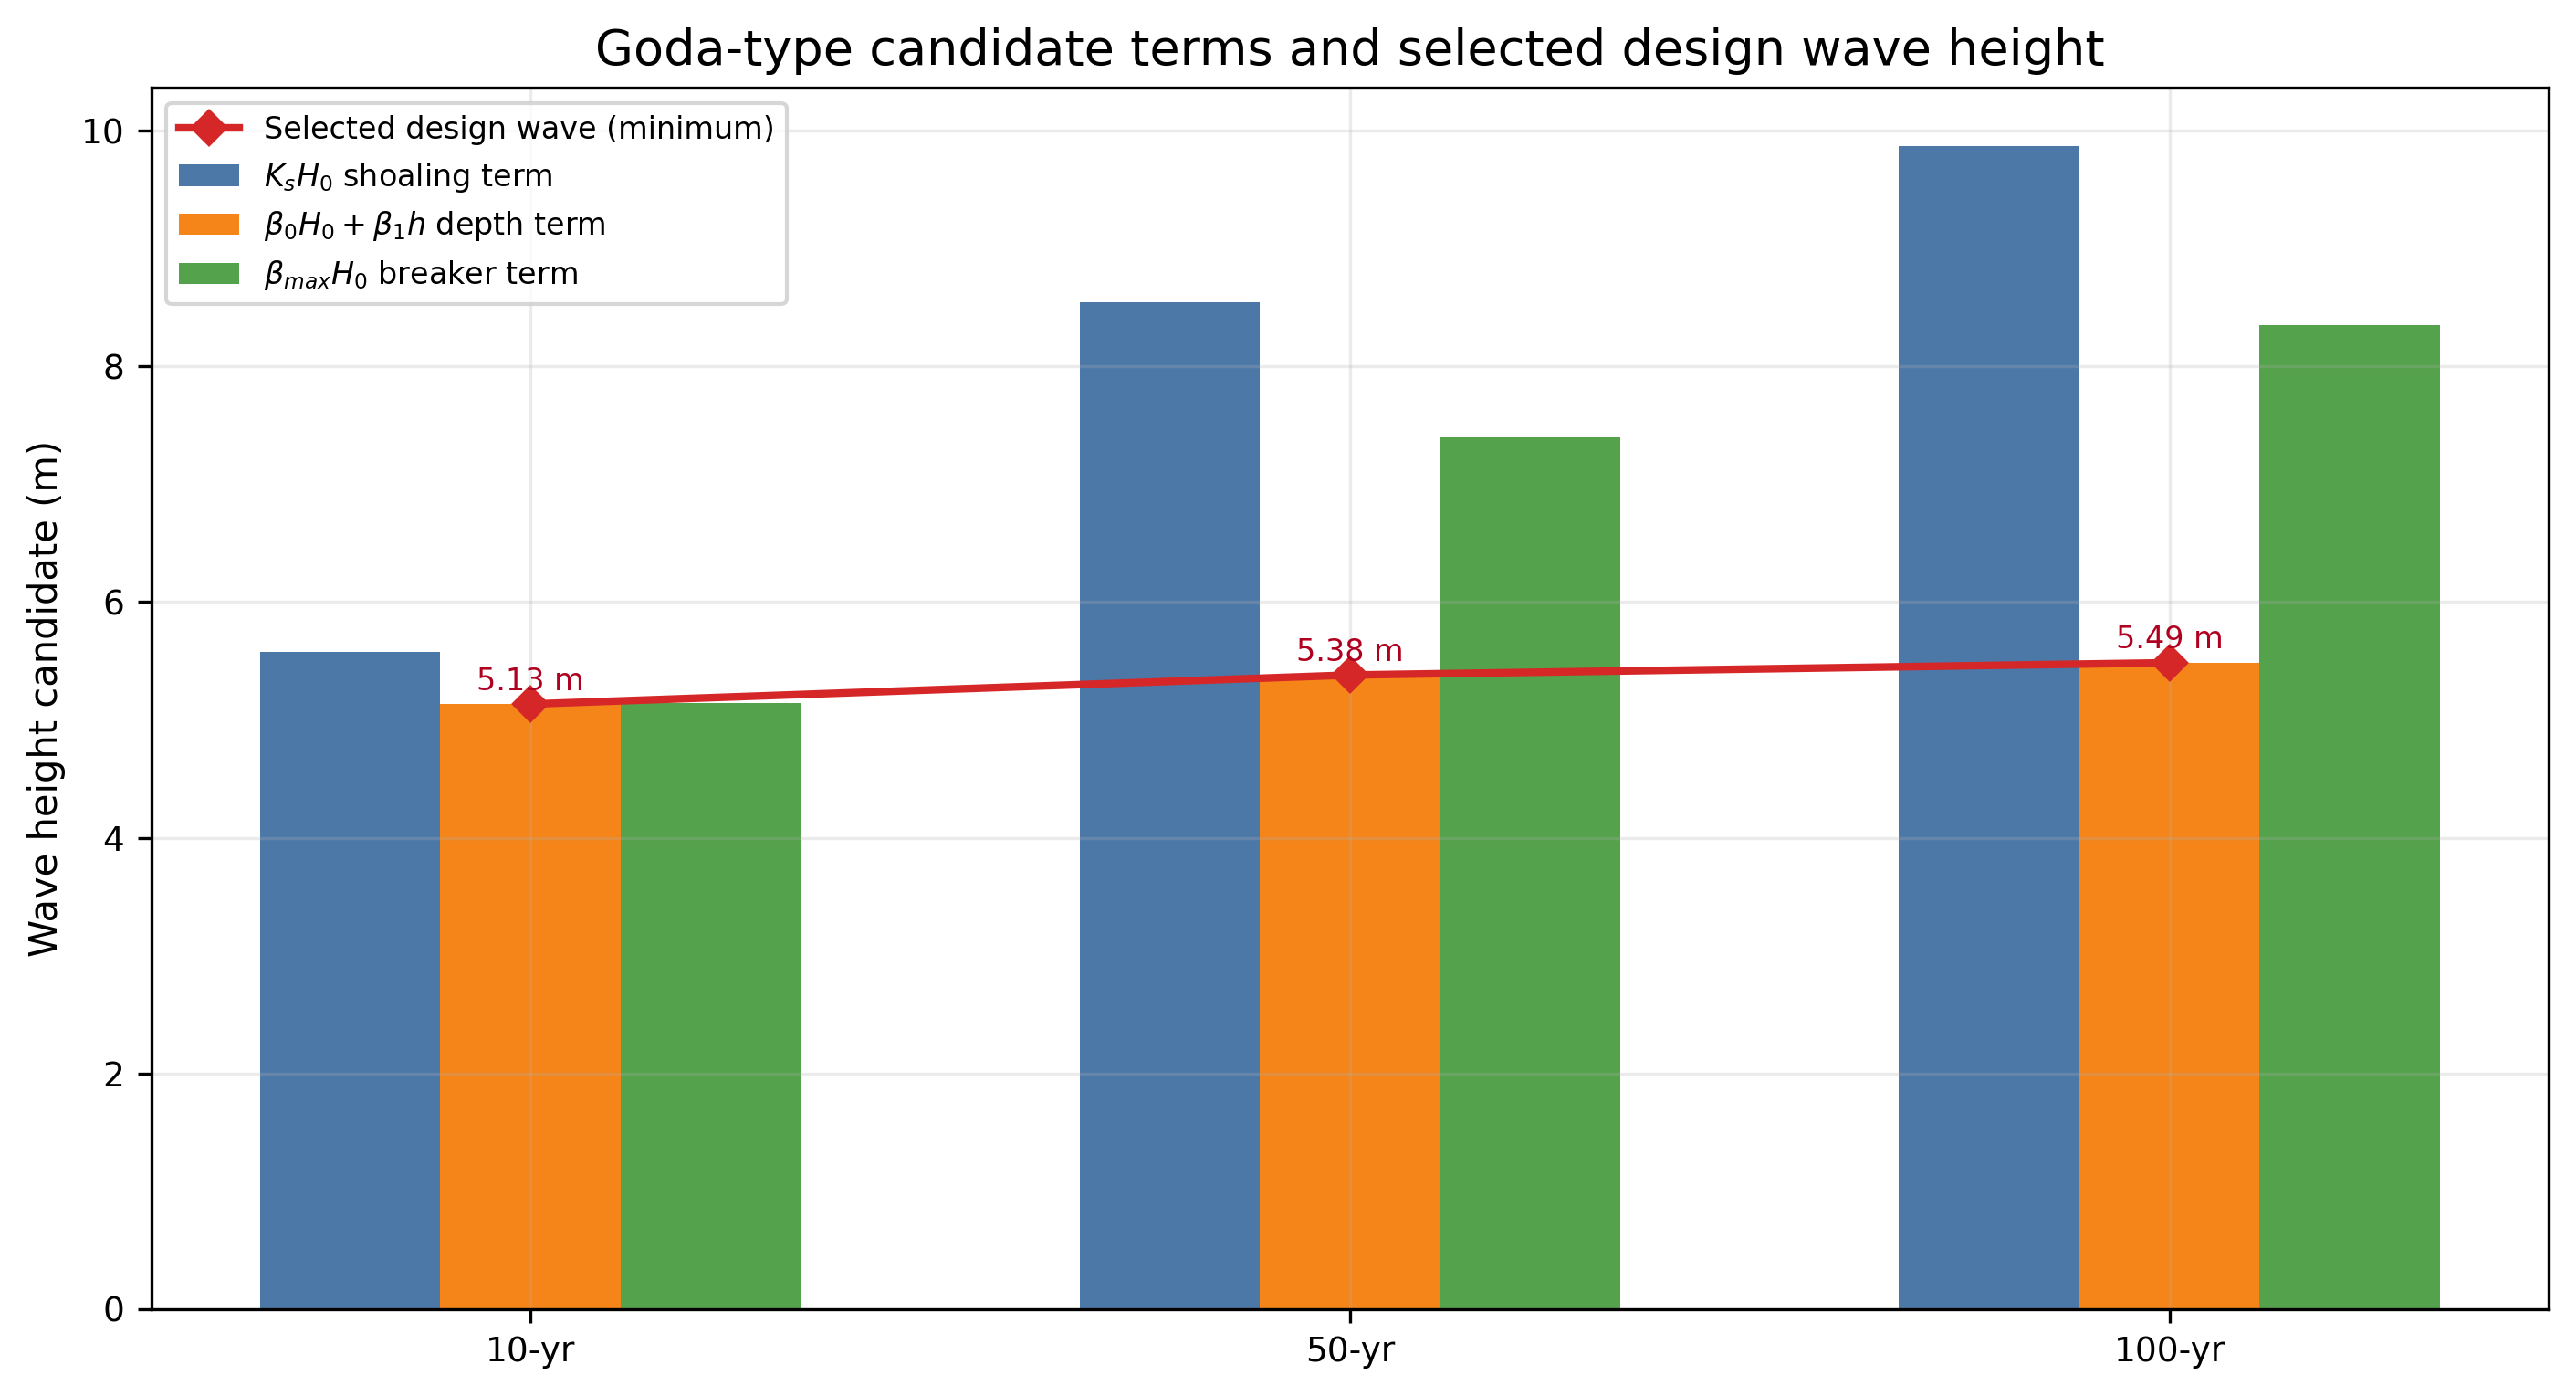
\includegraphics[width=0.94\textwidth]{figures/fig_6_goda_candidate_terms_enhanced.png}
\caption{Goda-type candidate terms and selected design wave height.}
\end{figure}

\begin{figure}[H]
\centering
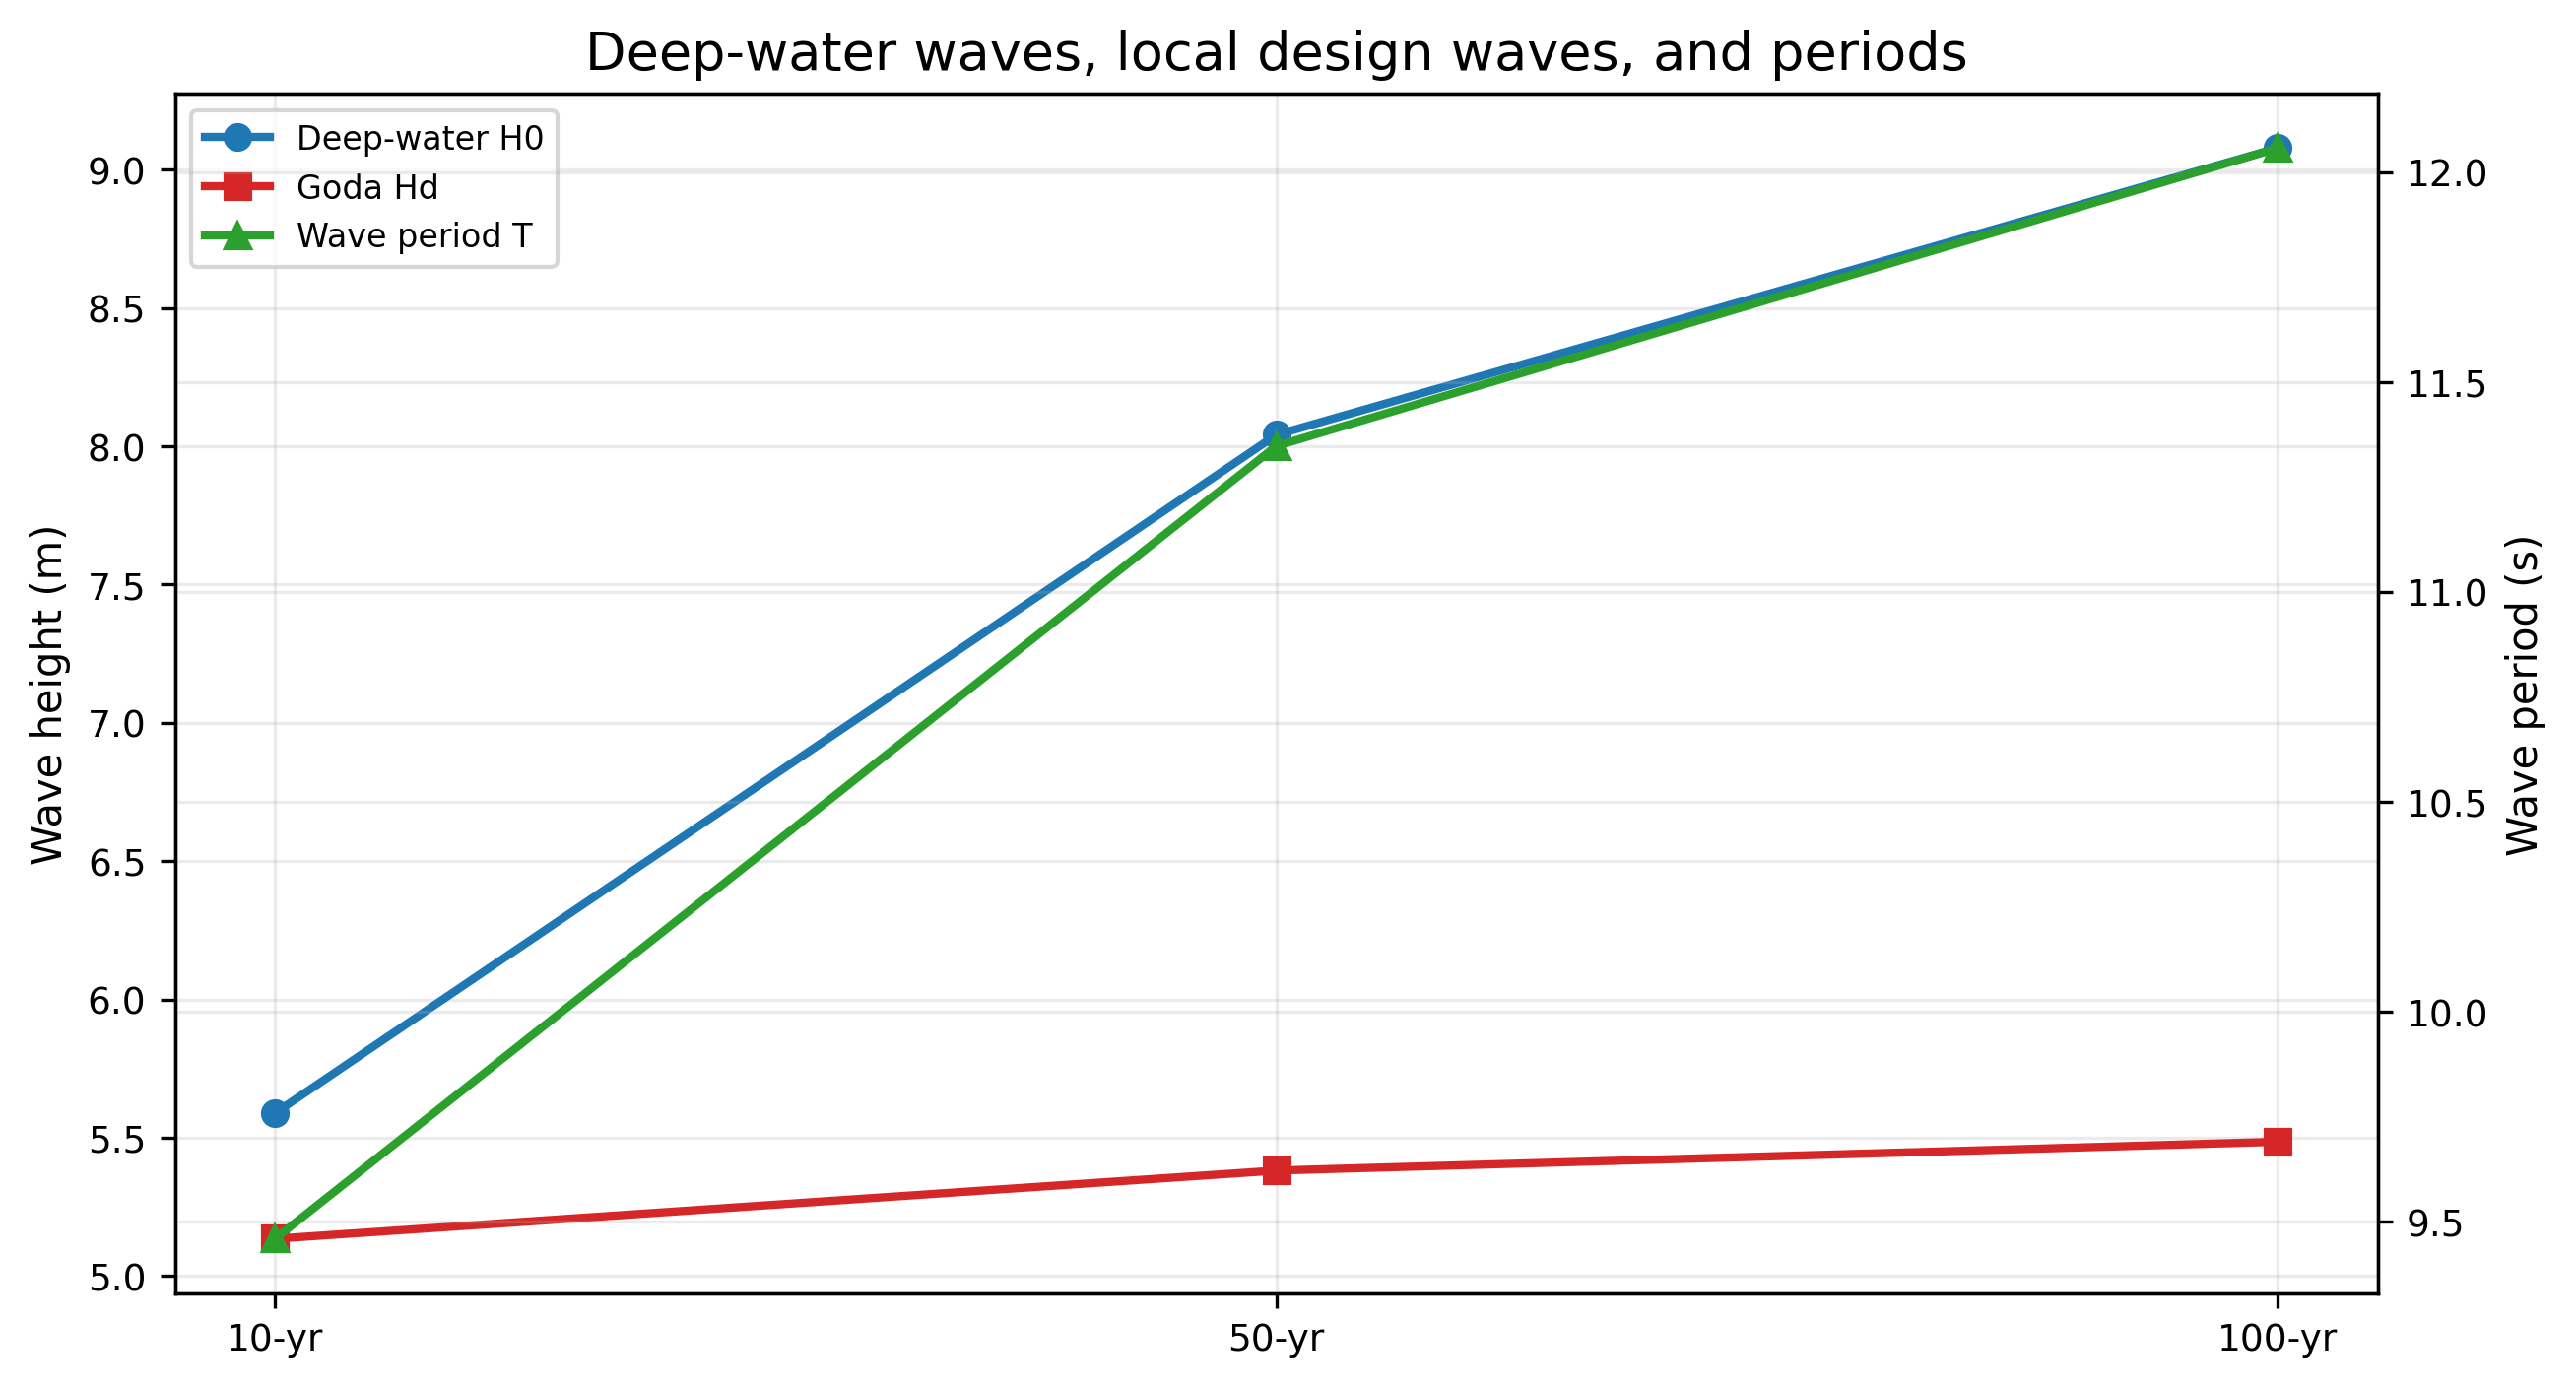
\includegraphics[width=0.90\textwidth]{figures/fig_7_wave_height_period_summary.png}
\caption{Comparison of deep-water wave height, local design wave height, and wave period.}
\end{figure}

\section{Final Design Summary}
\begin{table}[H]
\centering
\caption{Final preliminary design values.}
\begin{tabular}{lr}
\toprule
\textbf{Design item} & \textbf{Adopted/calculated value} \\
\midrule
Harbor type & Small commercial harbor \\
Maximum/design vessel length & 80 m \\
Maximum/design draft & 5.5 m \\
Maximum/design beam & 14 m \\
Quay wall length & 150 m \\
Turning basin diameter & 160 m \\
Navigation channel width & 70 m \\
Required navigation depth & 7.1 m \\
Perpendicular breakwater length & 575 m \\
Parallel breakwater length & 400 m \\
Total preliminary breakwater length & 975 m \\
10-year deep-water wave height, $H_{0,10}$ & 5.59 m \\
50-year deep-water wave height, $H_{0,50}$ & 8.04 m \\
10-year Goda design wave, $H_{d,10}$ & 5.13 m \\
50-year Goda design wave, $H_{d,50}$ & 5.38 m \\
Governing wave transformation condition & Depth-limited breaking \\
\bottomrule
\end{tabular}
\end{table}

\section{Conclusions}
\begin{enumerate}[leftmargin=1.0cm]
    \item A small commercial harbor layout was developed using a design vessel length of 80 m and design draft of 5.5 m.
    \item The required navigation depth is 7.1 m. Based on the linear bathymetry approximation, this depth occurs approximately 524 m offshore.
    \item The selected perpendicular breakwater length of 575 m reaches a local depth of about 8.1 m, so the breakwater reaches the required navigation depth. A navigation channel may still be marked or dredged for safe access, but the preliminary layout satisfies the depth requirement.
    \item The preliminary parallel breakwater length is 400 m, giving a total preliminary breakwater length of 975 m.
    \item The Goda-type design wave heights at the breakwater are 5.13 m for the 10-year return period and 5.38 m for the 50-year return period. For both cases, the governing condition is depth-limited breaking.
\end{enumerate}

\section{Limitations}
This is a preliminary academic design. The bathymetry is estimated from only two Google Earth Pro profile points, and the harbor layout is schematic rather than georeferenced. A final engineering design should use a detailed hydrographic survey, geotechnical data, wave transformation modelling, sedimentation assessment, navigational safety checks, and the exact coefficient set required by the course instructor.

\section{References and Data Sources}
\begin{enumerate}[leftmargin=1.0cm]
    \item CE480 Lecture Notes: Wave generation and prediction; JONSWAP wind-wave growth method.
    \item CE480 Lecture Notes: Wave climate and extreme-wave analysis.
    \item CE480 Lecture Notes: Wave transformation and Goda design wave height method for breakwater design.
    \item CE480 HW2 Group 3: Site selection and effective fetch calculation. Used for site coordinate, critical fetch directions, and effective fetch methodology.
    \item CE480 HW3 Group 3: JONSWAP wind-wave prediction from ERA5 wind data. Used for annual wave-height inputs and critical direction/fetch workflow.
    \item CE480 HW4 Group 3: Gumbel extreme wave analysis. Used for 10-year and 50-year deep-water design wave heights.
    \item Google Earth Pro profile points provided by the user: 1500 ft, -19 ft and 1.26 mi, -120 ft; converted to 457.2 m, 5.79 m depth and 2027.8 m, 36.58 m depth.
\end{enumerate}

\end{document}
